\chapter{Semi-automatic tracking of wave-type EODs}
\label{Methods}

\section{Introduction}

Clearly determining the causalities of animal behaviors in experimental or observational studies is often challenging, since animals are sensitive to a broad range of stimuli. Certain behaviors can, for example, be elicited by different social and environmental stimuli or be influenced by an animal's current internal state \citep{Chapman1995, Sapolsky2005, Boon2007, Markham2015}. Regarding all these influencing factors in a single scientific project is certainly difficult, if not impossible. Laboratory studies usually tackle this issue by reducing experimental environments and thereby the scope of factors potentially influencing behaviors (e.g. mice startle response, \citealp{Pantoni2020}; evoked communication in electric fish, \citealp{Bastianetal2001}). Such studies are, accordingly, most suitable to describe and evaluate causalities between specific behaviors and well defined stimuli in detail. On the other hand, their potential to discover unexpected behavioral traits and causalities is limited by their reduced experimental framework. Furthermore, since behaviors observed in the laboratory often deviate from those observed in the wild \citep{Cheney1995, Rendall1999, Henninger2018}, field studies or laboratory experiments with complex, more naturalistic designs are essential to gain a comprehensive understanding of an animal's natural behavior. Only in such settings the whole range of an animal's behavior can be observed and the validity of laboratory observations can be certified. 

The greatest challenge of such elaborate studies is the collection of comprehensive and viable data, including detailed observations of animals and their behaviors but also information about their surrounding environment. However, recent technological advances in remote recording techniques, tags, and data loggers allow for elaborate studies with freely moving and interacting animals in naturalistic settings \citep{Hughey2018, Mathis2018}. Recording devices got cheaper, smaller, and more energy efficient \citep{Hughey2018, Jolles2021} and our capabilities to analyze corresponding recordings greatly expanded and improved \citep{Dell2014}. A benefit of these approaches is that recordings contain rather unspecific data from which all sorts of information can be retrieved after the recordings have been made, including behavioral events or environmental information \citep{Gomez2014}. 

% Bio-loggers
Based on the requirements of a scientific project, i.e. model species, environmental conditions, and the scientific question, the most suitable recording technique can be selected from a huge variety of available devices \citep{Hughey2018}. For example, in studies on highly mobile animals or those who live in remote, hard to access areas, bio-loggers are most suitable to collect viable behavioral data \citep{Nagy2010, StrandburgPeshkin2017}. Bio-loggers are small recording devices that get affixed to animals themselves and can be equipped with a variety of different on-board sensors, like GPS, magnetometers, pressure sensors, microphones or even video cameras \citep{Hughey2018}. With the help of bio-loggers, many interesting insights into different aspects of natural animal behavior have already been gained, including collective movement \citep{Nagy2010, Strandburg2015}, leadership \citep{Strandburg2018}, or foraging ecology of deep-diving animals (elephant seals, \citealp{Robinson2012}).

Nevertheless, in studies utilizing bio-loggers, experimenters frequently need to interact with animals (e.g. to mount, recharge, or read-out loggers) and animals are required to carry recording devices. This alone already can result in changes of behaviors, reproduction, or survival, and thus bias observations \citep{Saraux2011}. In order to reduce these biasing factors, different trade-offs regarding sample rate, duty cycling, and battery life are required \citep{StrandburgPeshkin2017, Hughey2018}. Furthermore, not all individuals of a study population can usually be equipped with recording devices (e.g. \citealp{StrandburgPeshkin2019}) and those loggers deployed are limited in their recording range to the direct surrounding of the respective animal. Accordingly, bio-loggers can potentially miss out on recording relevant stimuli that elicit recorded behaviors when  (i) stimuli take place off recording cycle or (ii) out of detection range of deployed devices, with the latter also including (iii) untagged animals. 

% Remote sensing
An alternative approach for behavioral studies in naturalistic, open space environments is to detect and track animals and their behaviors in external recordings \citep{Kuhl2013, Hughey2018}. Since interactions with animals are not required for this approach, external influences on their behaviors are minimized \citep{Saraux2011}. Furthermore, the range of feasible behavioral studies is extended to also include animal species that are hard or impossible to access. For example, herds of caribous have remotely been filmed using unmanned aerial vehicles like drones and analyzed in the context of collective movement and information transfer in groups \citep{Torney2018}, individual flight paths of bats and birds have been reconstructed from video recordings of stationary cameras \citep{Theriault2014}, and electric signals of electric fish have been recorded using electrode arrays submerged in the water and analyzed to gain insights into their natural communication and movement behaviors \citep{Henninger2018, Henninger2020}. 

% animal biometrics
However, the analysis of such recordings is way more challenging compared to bio-logger approaches. The methods comprised in a ``biometric system'' usually include algorithms to detect certain animal biometrics, i.e. manifestations of an animal's appearance and/or behavior in such recordings, and compare them to predefined biometric profiles corresponding to the typical manifestation of these biometrics in, for example, a certain species, individual, or behavior \citep{Gaston2004, Sherley2010, Kuhl2013}. In order to enable reliable classification, utilized biometrics need to be universally displayed, while showing sufficient variation between biometric profiles. For example, coat patterns of zebras \citep{Lahiri2011} or the configuration of dark spots on penguin bellies \citep{Sherley2010} are suitable biometrics to reliably identify individuals (biometric profiles). Yet already the reliable detection of selected animal biometrics can be challenging, since individuals can temporarily leave observation areas or the detection of biometrics may fail because of low signal-to-noise-ratios. Further algorithmic challenges can arise from ambiguous biometric profiles. The selection of animal biometrics that can be extracted from recordings is usually limited, which potentially reduces the specificity of biometric profiles. Because of these limitations, biometric profiles are often time-variant and/or overlap in their characteristics, e.g. when using an animal's spatial position for individual identification and tracking (e.g. \citealp{Madhav2018}).

% Electric fish
Based on the general idea of a biometric system, we developed methods and algorithms capable of tracking individual behaviors in freely moving groups of the electric fish \Lepto{}. These fish produce a semi-sinusoidal electric field through continuous discharges of an electric organ (EOD, \citealp{Turner2007}) used for electrolocation \citep{Fotowat2013} and communication \citep{Albert2005, Smith2013}. In order to track electric signals of individual fish, we take advantage of the different characteristics of their EODs that can be extracted from recordings of electrode arrays submerged in the water \citep{Jun2013, Madhav2018, Henninger2018, Raab2019}. 

Previous approaches already tracked electric signals of individual fish by means of their individual specific EOD frequency (EODf, \citealp{Henninger2020}) or spatial electric field properties that can be reconstructed from signal powers across recording electrodes \citep{Madhav2018}. However, the latter depends on the fish's spatial position and orientation and even though individual specific EODfs are remarkably stable over minute to hours \citep{Moortgat1998}, they are sensitive to temperature changes and can be altered actively in the context of communication \citep{Dunlap2000, Smith2013}. Accordingly, these signal features can temporarily overlap between individuals, which complicates reliable tracking, especially for recordings of electric fish in high densities.

In the following sections, we describe and evaluate a new approach for analyzing the electric signals of whole populations of wave-type electric fish recorded with electrode arrays in different configurations. By combining, refining, and extending previous approaches, our algorithm is capable of tracking EODs of individual fish with unprecedented accuracy. Since various different behavioral traits of these fish, including communication \citep{Smith2013} and movement behaviors \citep{Madhav2018}, can be evaluated base on their EODs, our algorithms are a fundamental advancement for various different behavioral studies on freely moving and interacting electric fish \citep{Raab2019, Raab2021}.

\section{Data acquisition}

We developed an easy to modify recording setup that can be adapted, scaled, and adjusted according to the conditions of different experimental settings, e.g. varying environments or observation areas. All recording setups described below are powered by car batteries (12\,V, 80\,Ah) which reduces the influence of electric noise of line current and enables recordings even in hard to access areas, e.g. remote rivers in South America. The core element of the setup is its array of monopolar electrodes at low-noise buffer headstages (1$\times$gain, 10$\times$5$\times$5\,mm$^3$, \subfigrefb{setup_n_trace}{B}) arranged in grid-like structures (\subfigref{setup_n_trace}{C, D}). Electric signals are amplified (100$\times$gain, 100\,Hz high-pass filter, 10\,kHz low-pass), digitized at 20\,kHz with 16 bit resolution, and stored on external data storage devices for later offline analysis. Various electrode grid configurations have already been successfully applied to record populations of electric fish in the wild (\citealp{Henninger2018, Henninger2020}, unpublished field-trips: Colombia 2016, 2019, \subfigrefb{setup_n_trace}{C, E}), as well as in the laboratory (\citealp{Raab2019, Raab2021}, \subfigrefb{setup_n_trace}{D, F}). While the core element of the recording setup with its multiple electrodes and the configuration of amplifiers have remained unaltered during about a decade of electrode-grid based electric fish research, the hardware used for data handling and storage has been revised and improved along the way. The initial computer-amplifier system has been replaced with a more convenient and easy to operate system based on a Raspberry Pi (npi-electronics GmbH, Tamm, Germany, \subfigrefb{setup_n_trace}{A}). The recording software has also remained similar over the years except for being ported from C++ (\url{https://github.com/bendalab/fishgrid}) to Python 3.8 (\url{https://whale.am28.uni-tuebingen.de/git/raab/Rasp_grid.git}) and being more intuitive to handle, e.g. recording configurations can be set using a GUI.

\begin{figure}[h!]
  \centerline{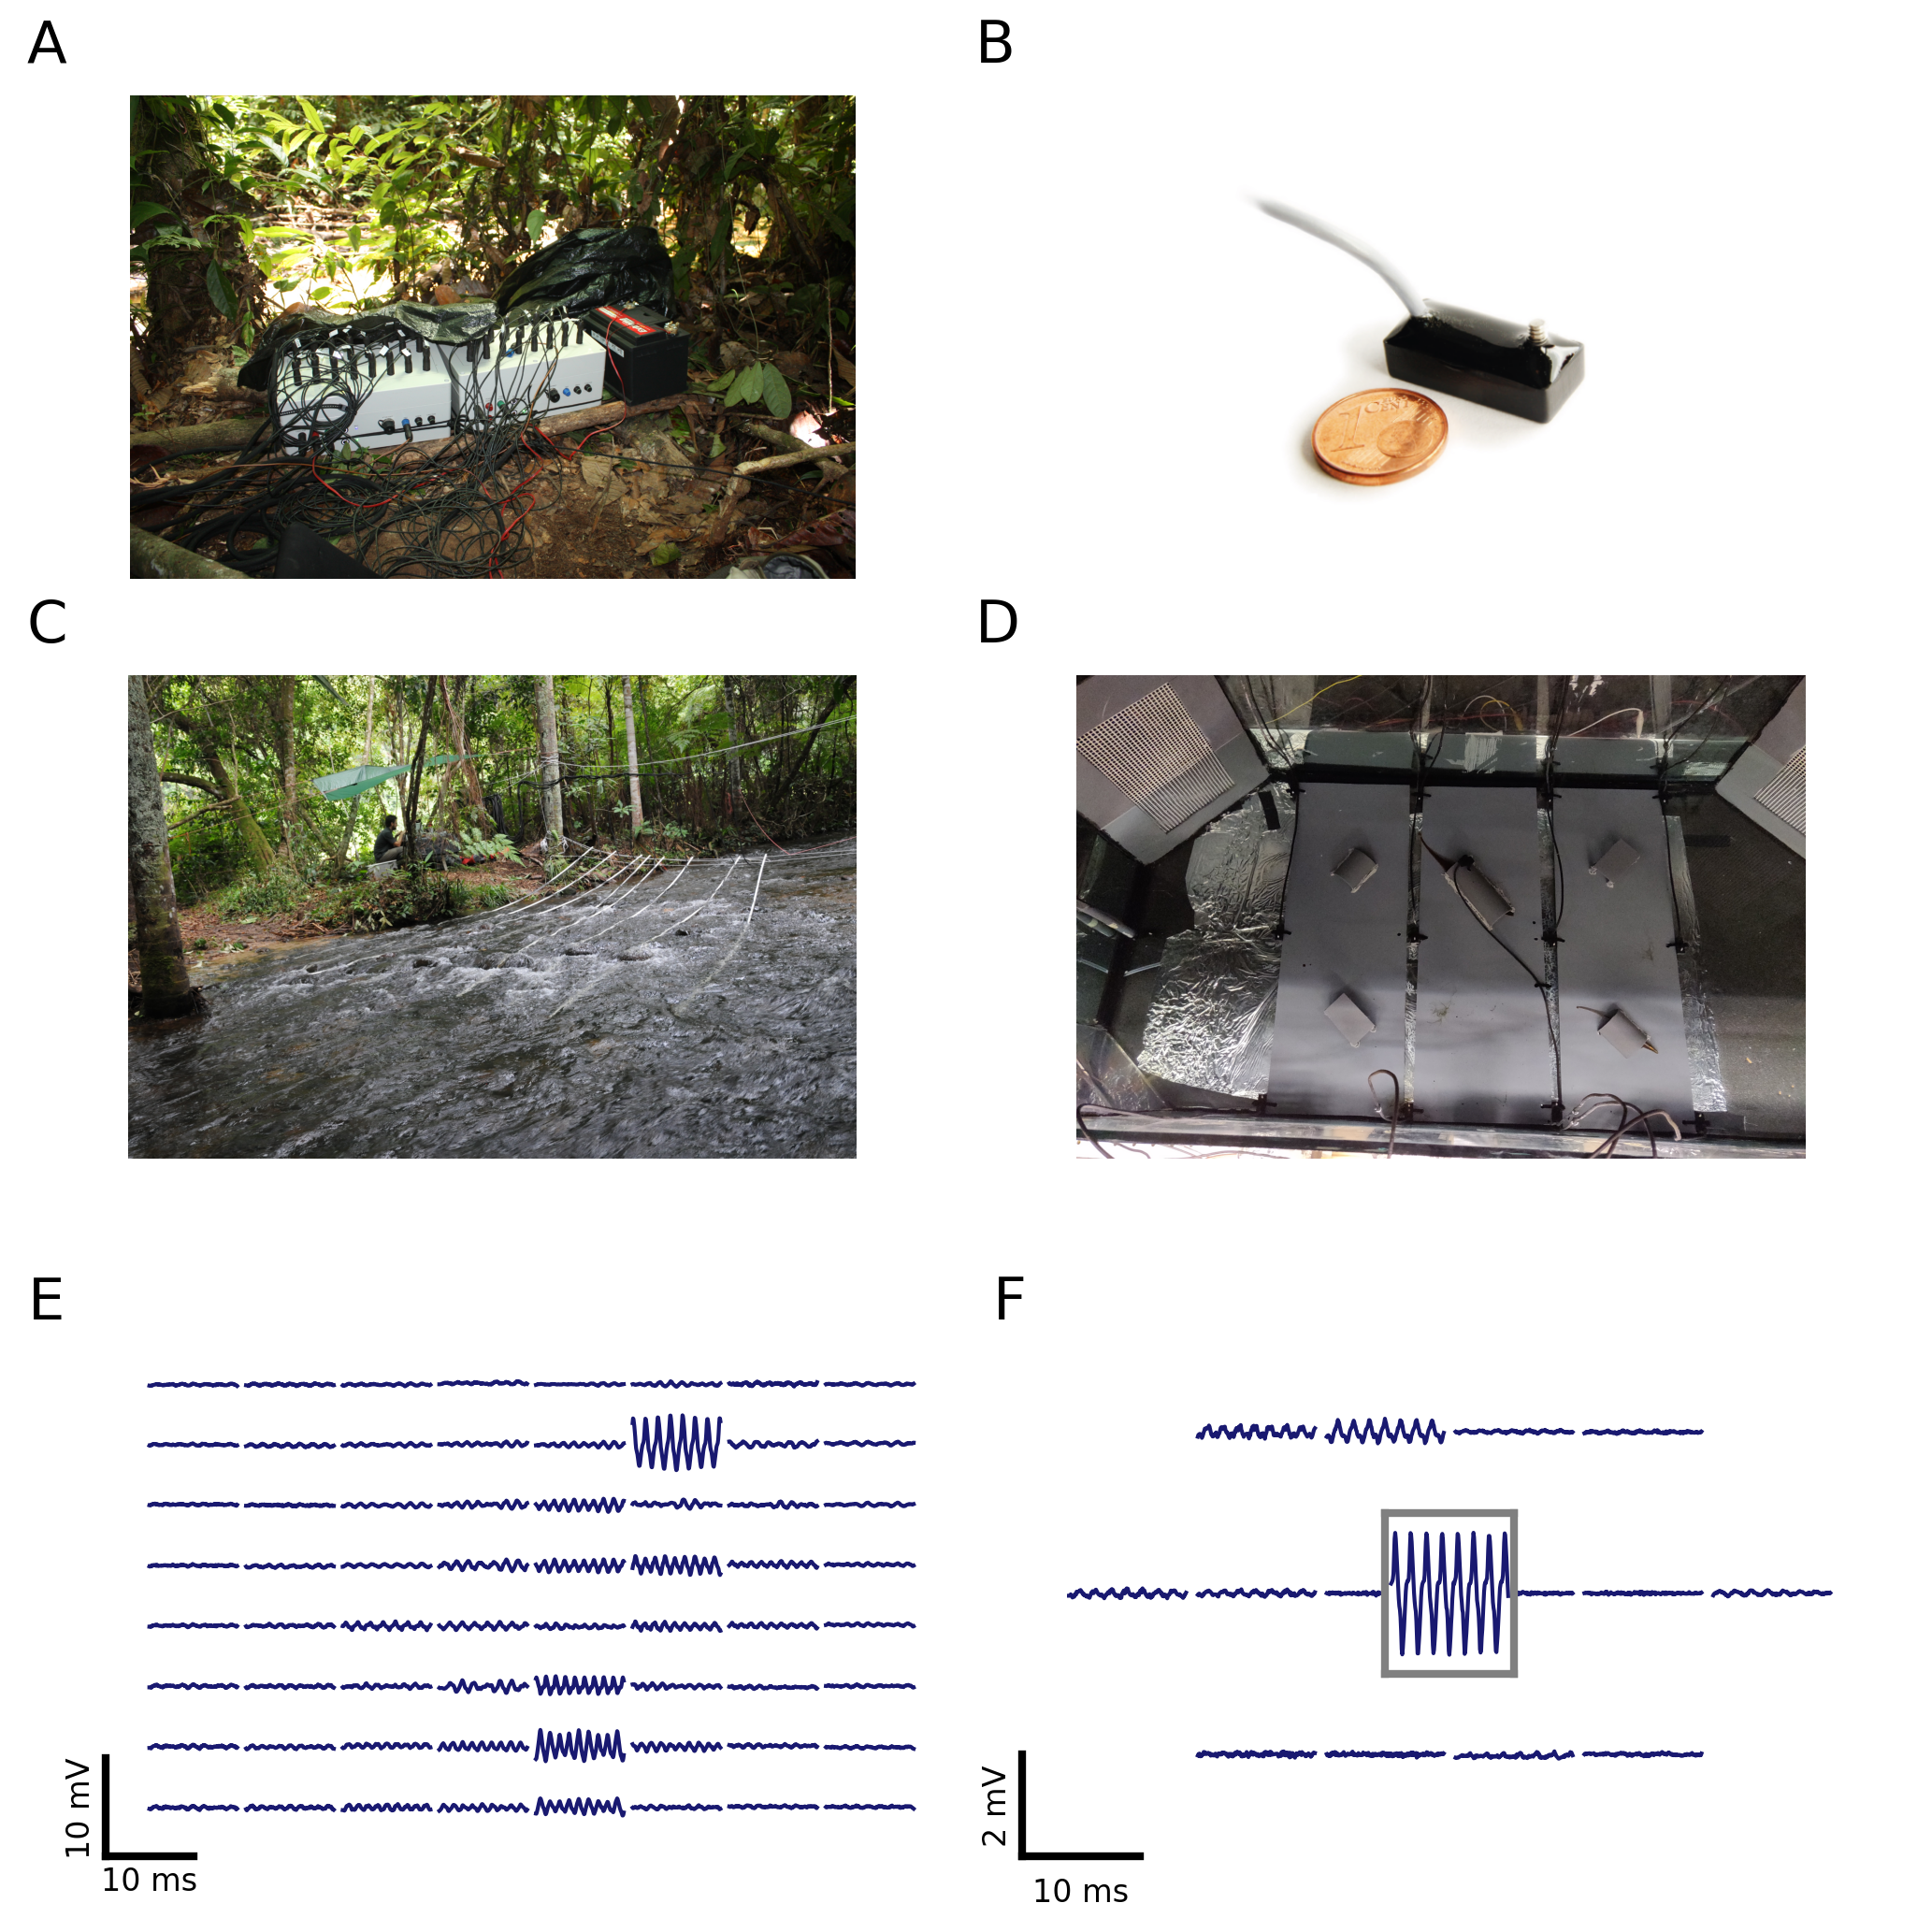
\includegraphics[width=.8\linewidth]{setups_and_raw_traces_new}}
%  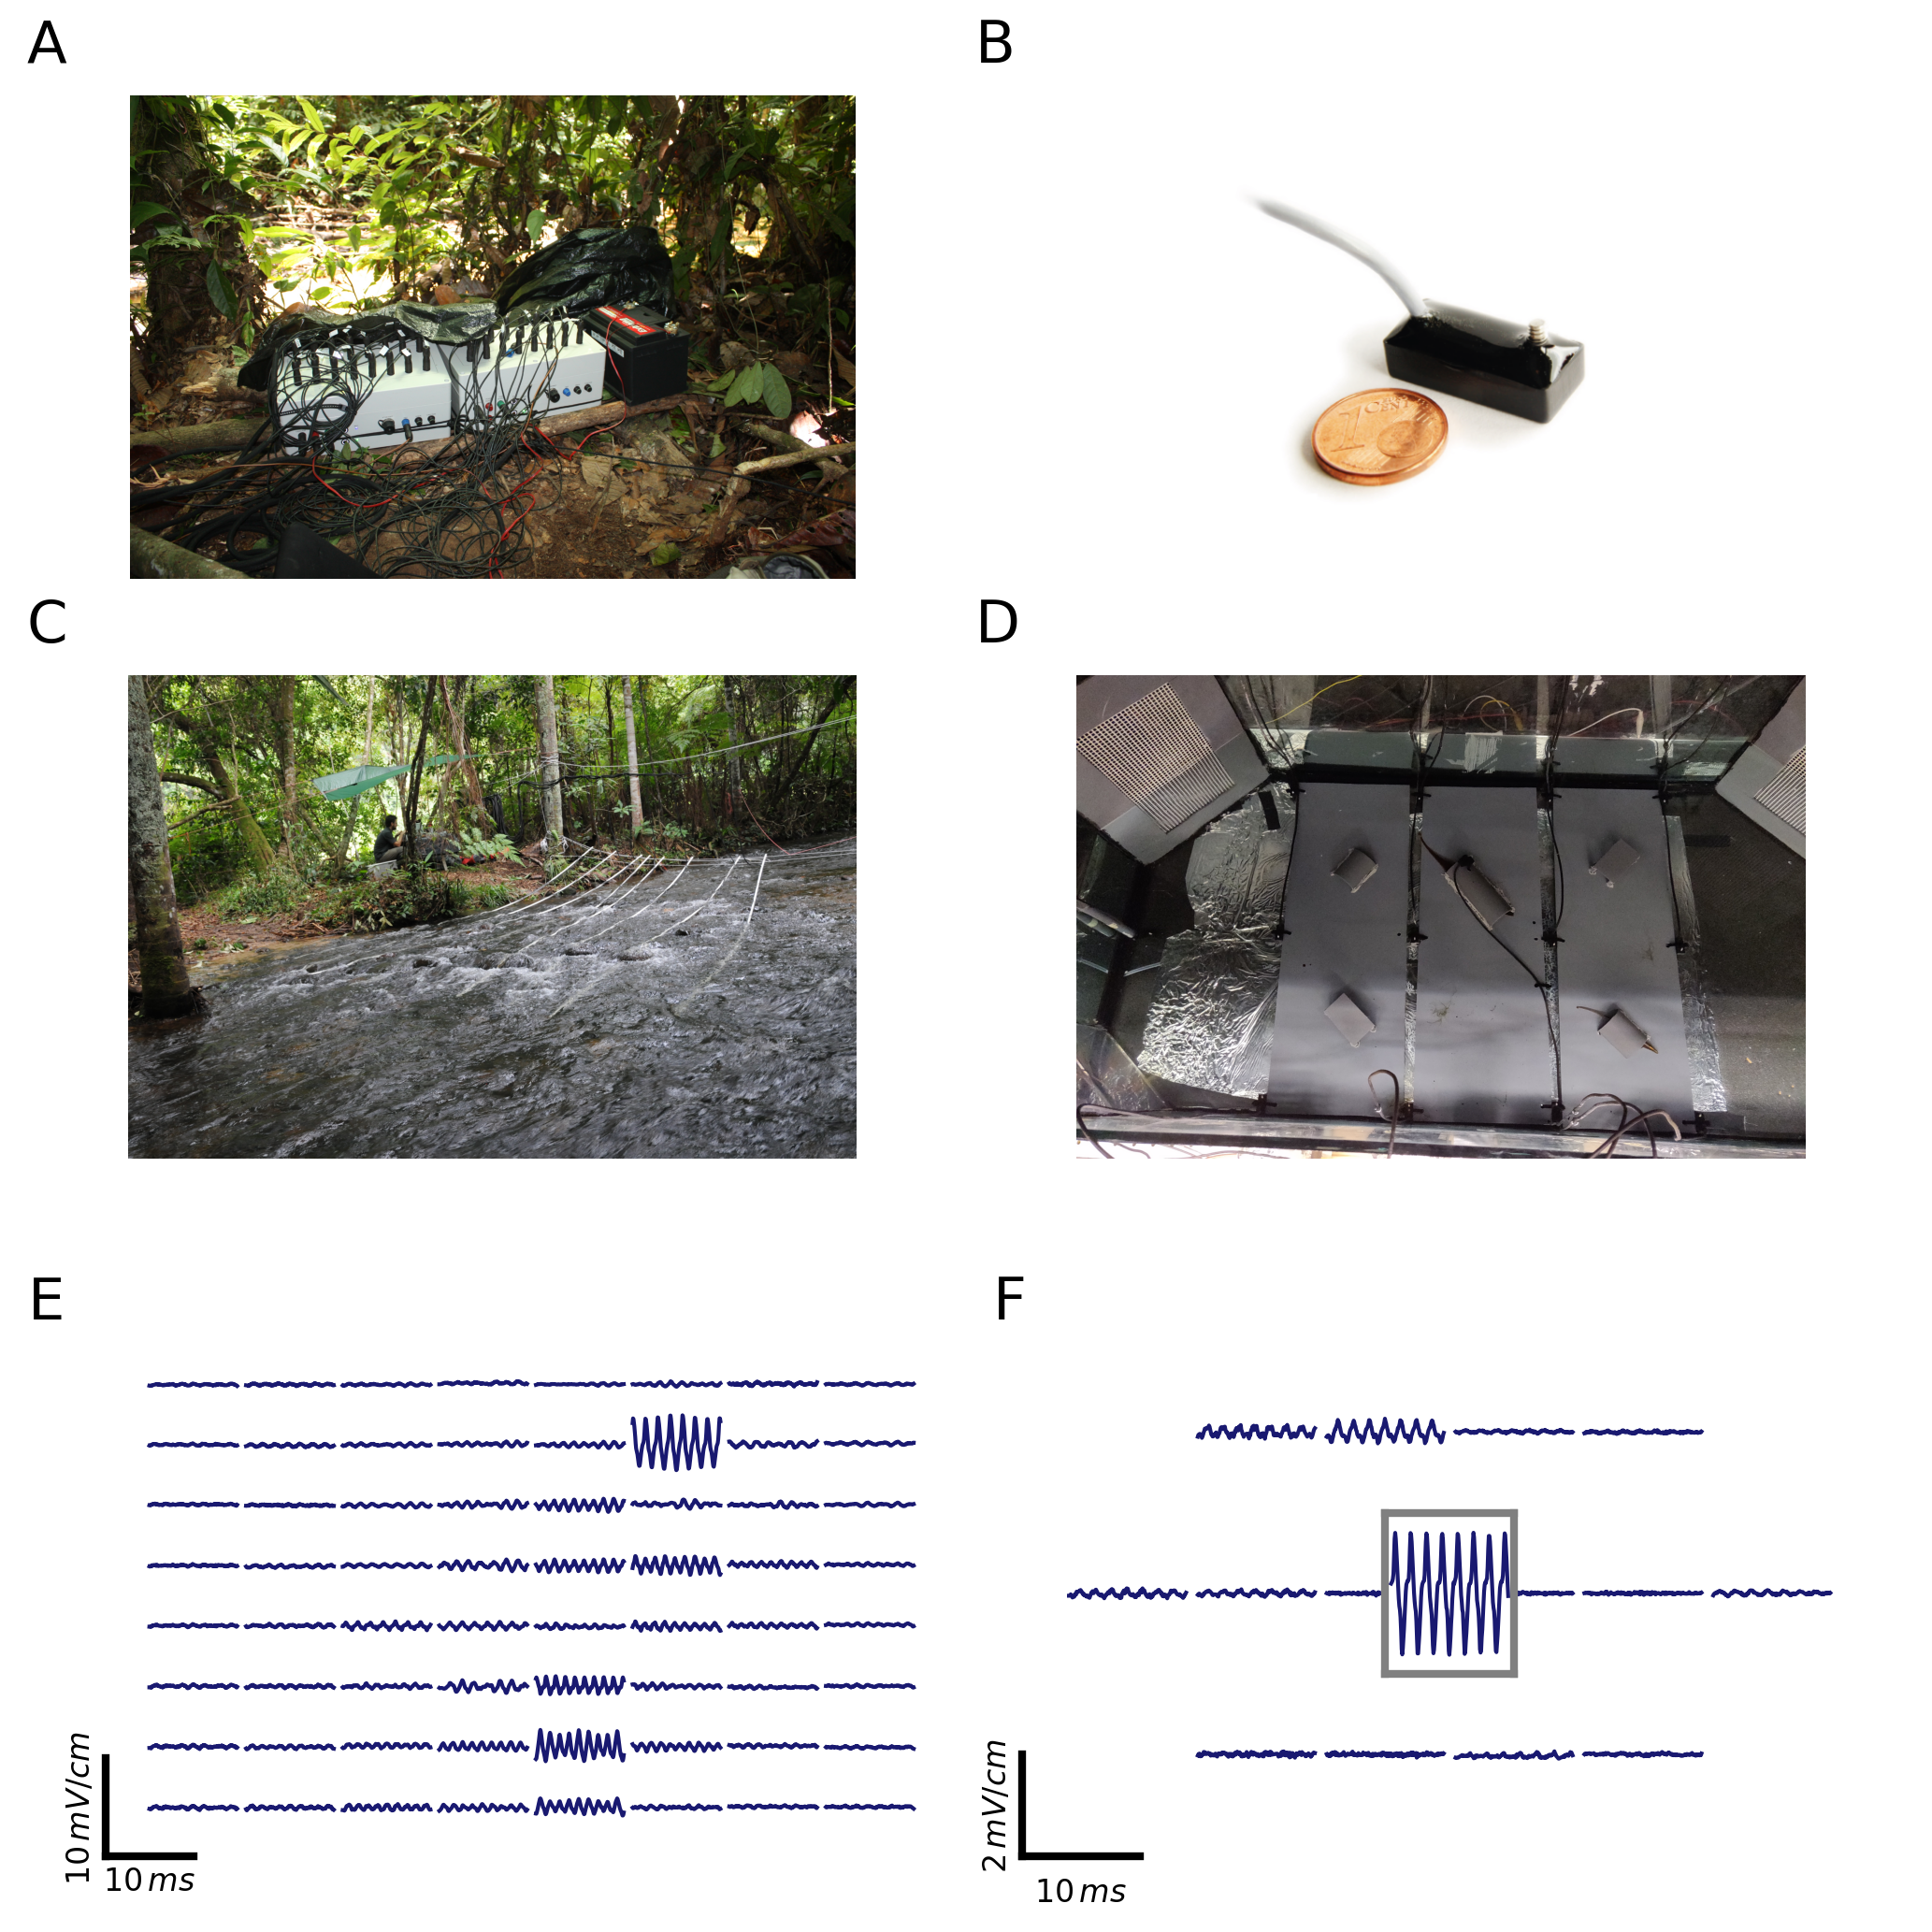
\includegraphics[scale=0.75]{setups_and_raw_traces}
  \caption{\label{setup_n_trace} Recording systems, electrode arrangements, and corresponding signals of recorded electric fish. \figitem{A} The latest version of the recording system enabling simultaneous recording with 16 electrodes. \figitem{B} Monopolar recording electrodes used for recordings in the field and laboratory experiments (after \citealp{Henninger2015}). \figitem{C} Recording setup used to record a population of \lepto{} in the Rio Rubiano, Colombia, in 2016. 64 electrodes were mounted on PVC-tubes and arranged in a 8$\times$8 grid covering an area of 3.5$\times$3.5\,m$^2$. \figitem{D} Recording setup used to record electric signals of pairs of \lepto{} during competitions in a laboratory experiment. 15 electrodes were equally distributed throughout the aquarium to ensure continuous detection of both individual's electric fields. \figitem{E} Snapshot of the electric signals recorded in Rio Rubiano, Colombia, in 2016 with the setup shown in panel~\panel{C}. \figitem{F} Snapshot of electric signals emitted during dyad interactions of \lepto{} in the competition experiment shown in panel~\panel{D}. The signal framed in grey corresponds to the signal recorded by the central electrode located in the long tube in the center of the aquarium (panel~\panel{D}). The EOD of the corresponding \lepto{} shows the characteristic shoulder in each EOD period.}
\end{figure}

%\section{Signal extraction and tracking}
%
%\subsection{Signal extraction}

\section{Detection of individual electric signals (EODs)}

EODs of individual fish are identified and extracted from the electric recordings based on their EODf and respective harmonic structure (\subfigref{signal_extraction}{C}). For each electrode, we compute power spectral densities (PSDs) of overlapping data snippets shifted by $\Delta t$\,$\approx$\, 300\,ms (\subfigref{signal_extraction}{A}). The size of fast Fourier transform windows (nfft) and their overlap represent the trade-off between frequency and temporal resolution. In our analysis, we set both parameters to obtain a temporal resolution of $\Delta t$\,$\approx$\, 300\,ms according to the formula
\begin{equation}
\Delta t = \frac{\text{nfft}}{f_s} \cdot (1-\theta) 
\end{equation}
with nfft being the size of the fft-windows, $f_s$ the sampling-rate of the recording electrodes, and $\theta$ the overlap fraction of fft-windows. 

When we aim for reliable and continuous EODf detection in recordings featuring fish in high density, large fft-windows with more overlap (nfft$=2^{16} \approx$  3.28\,s; $\theta$ = 0.9) are required to resolve EODf differences occasionally dropping below 1\,Hz (e.g. \citealp{Raab2019}). In contrast, smaller fft-windows with less overlap are more suitable when the temporal resolution of electrocommunication signals is prioritized, e.g. in recordings of dyad interactions during competitions (nfft$=2^{15} \approx  1.64$\,s; $\theta$ = 0.8, \citealp{Raab2021}). 

In order to detect the individual specific EODfs of all recorded fish simultaneously, we sum up PSDs referring to the same time point (t$_i$) across electrodes (\subfigref{signal_extraction}{B}). Peak frequencies are detected in the summed up PSDs after logarithmic transformation \citep{Todd1999, Henninger2020} using the formula
\begin{equation}
L = 10 \cdot log(P/p_0)
\end{equation}
with $P/p_0$ being the powers of frequency ($P$) in the Fourier transformed data relative to a reference power of $p_0 = 1$. 

Detection groups comprising fundamental frequencies and at least two harmonics are assembled from these detected peak frequencies, beginning with the peak frequency featuring the higher spectral power (\subfigrefb{signal_extraction}{C}, \citealp{Henninger2020}). The peak detection as well as the extraction of detection groups is described in detail in \citet{Henninger2020}. 

Each detection group extracted from the summed up PSDs at time $t_i$ corresponds to one signal $k$. For the subsequent signal tracking, different signal features 

\begin{equation}
 \vec{X_{k, i}} = (f_{k,i}, L_{k, i, 1},  ..., L_{k, i, n})
 \label{signal_features}
\end{equation}

are extracted for each signal $k$ detected at time step $i$, including its fundamental EODf ($f_{k,i}$) and the corresponding logarithmic powers ($L_{k, i, n}$) in the PSDs of all $n$ recording electrodes. 

\begin{figure}[p]
  \centerline{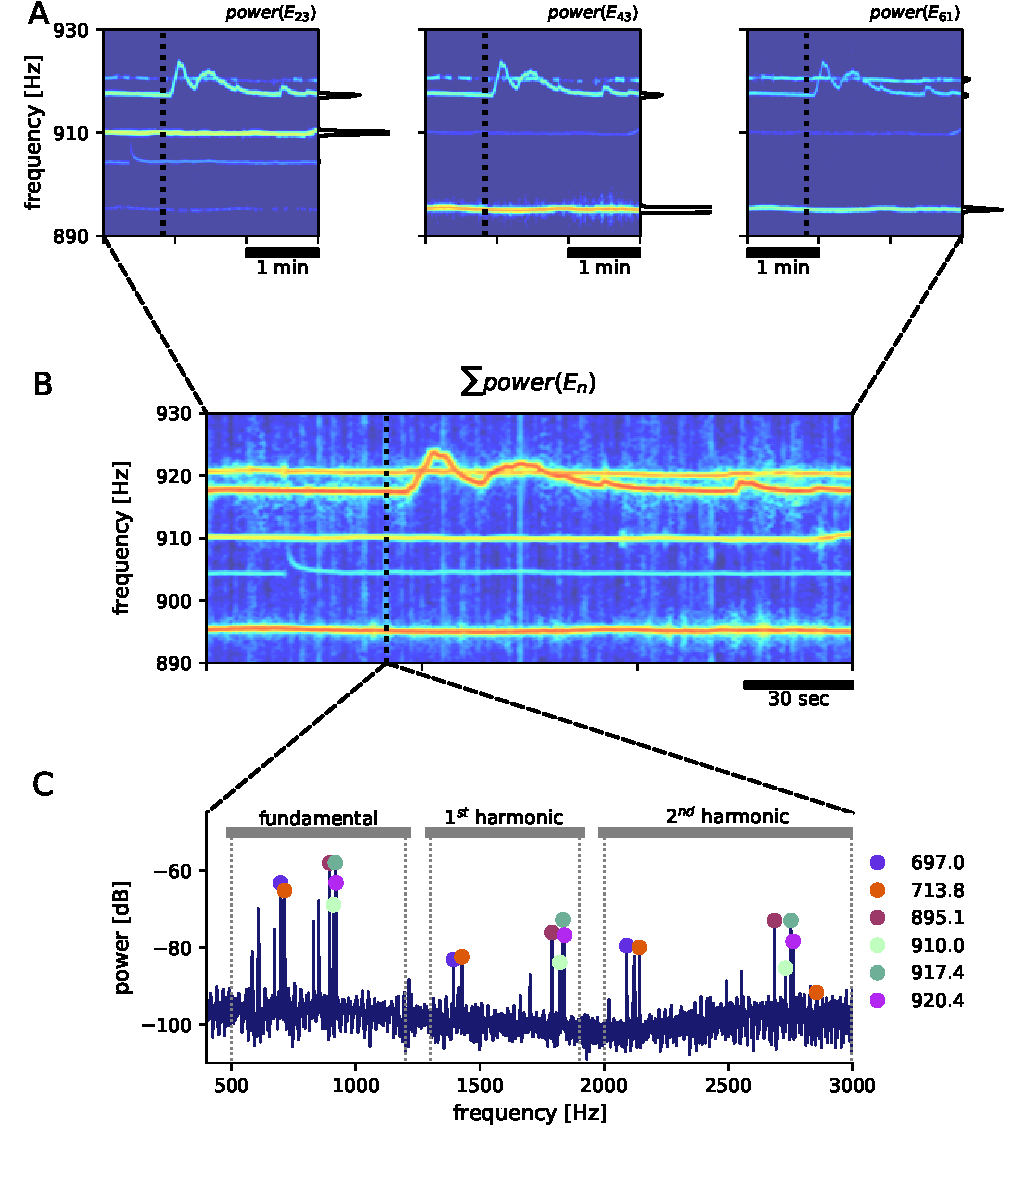
\includegraphics[width=.9\linewidth]{signal_extraction}}
%  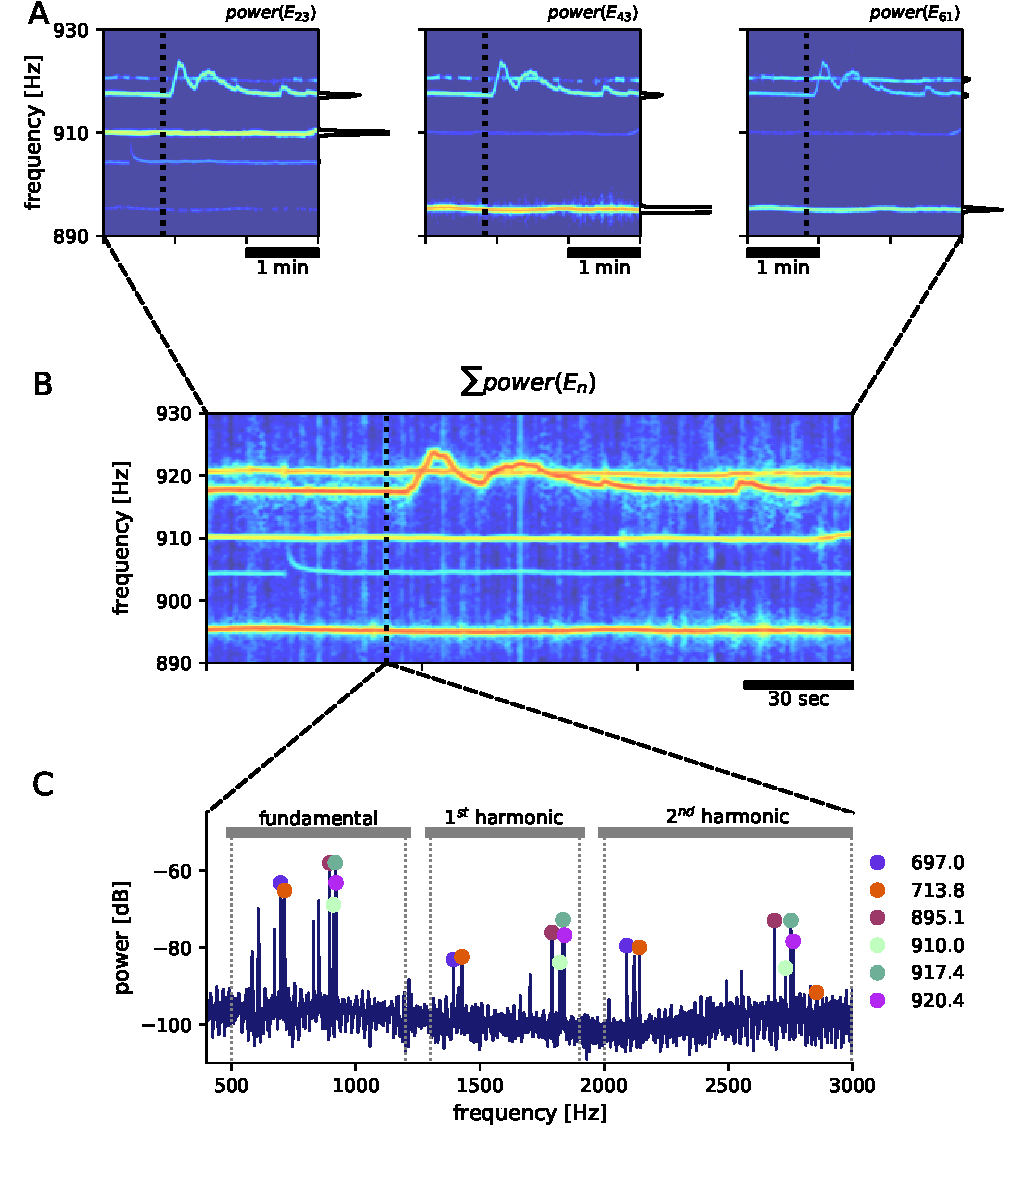
\includegraphics[scale=0.75]{signal_extraction}
  \caption{\label{signal_extraction} EOD frequency extraction from electric recordings obtained with an electrode array consisting of 8$\times$8 electrodes during the day of the 10$^{th}$ of April, 2016 in Colombia. \figitem{A} Spectrograms of a representative 3\,min  data snippet recorded on three example electrodes. Warmer colors represent increased power in respective frequencies. EODfs of individual \lepto{} remain rather stable, unless altered intentionally when emitting communication signals (see EODf trace starting at $\sim$~917\,Hz). A non-logarithmic PSD extracted at the time (50\,s) indicated with the dotted line is shown at the side of each panel. \figitem{B} By summing up spectrograms of all electrodes, more clear EODf traces can be obtained. \figitem{C} We detect frequency peaks in these summed up powerspectra and assign them into frequency groups corresponding to individual fish. A frequency group consists of an individual's fundamental EODf and at least two harmonics (see \citealp{Henninger2020}). Fundamental EODfs, their corresponding powers in the power spectra of all individual electrodes and their detection times are stored for the subsequent EODf tracking. } 
\end{figure}

%\subsection{Tracking wave-type electric fish signals}
\section{Tracking individual electric signals (EODs)}

For tracking individual EODs, we follow the approach of feature comparison. Previous approaches compare either EODf or signal power across electrodes over time \citep{Madhav2018, Henninger2020}. However, both of these signal features are time-variant and can potentially overlap between fish. EODf can be actively altered in the context of communication \citep{Smith2013} and the signal powers across electrodes change with the fish's motion \citep{Madhav2018}. This variability and potential overlap in signal features complicates reliable tracking, especially when fish are recorded in high abundance. Furthermore, existing algorithms tracking signals in order of their temporal detection, i.e. signals detected in consecutive time steps are assigned to already tracked EODf traces comprising preceding signals, potentially leads to tracking errors and accuracy limitations. Even with the utilization of an electrode array, EODs of freely moving and interacting electric fish are rarely detected continuously. Low signal-to-noise ratios, resulting from large distances between fish and recording electrodes or environmental conditions distorting electric fields, frequently lead to detection losses. When multiple fish with similar EODfs are recorded simultaneously, EODf traces can potentially cross each other (e.g. in the context of emitted communication signals, \citealp{Smith2013}). Especially in these occasions, detection losses can frequently result in tracking errors. 

In order to circumvent this issue, we developed a tracking algorithm which, first, uses a compound signal error including both differences in EODf and signal power across electrodes as tracking feature (\figref{features}) and, second, is less constrained by the temporal detection of signals (\figref{tmp_tracking}). 

\begin{figure}[h!]
  \centerline{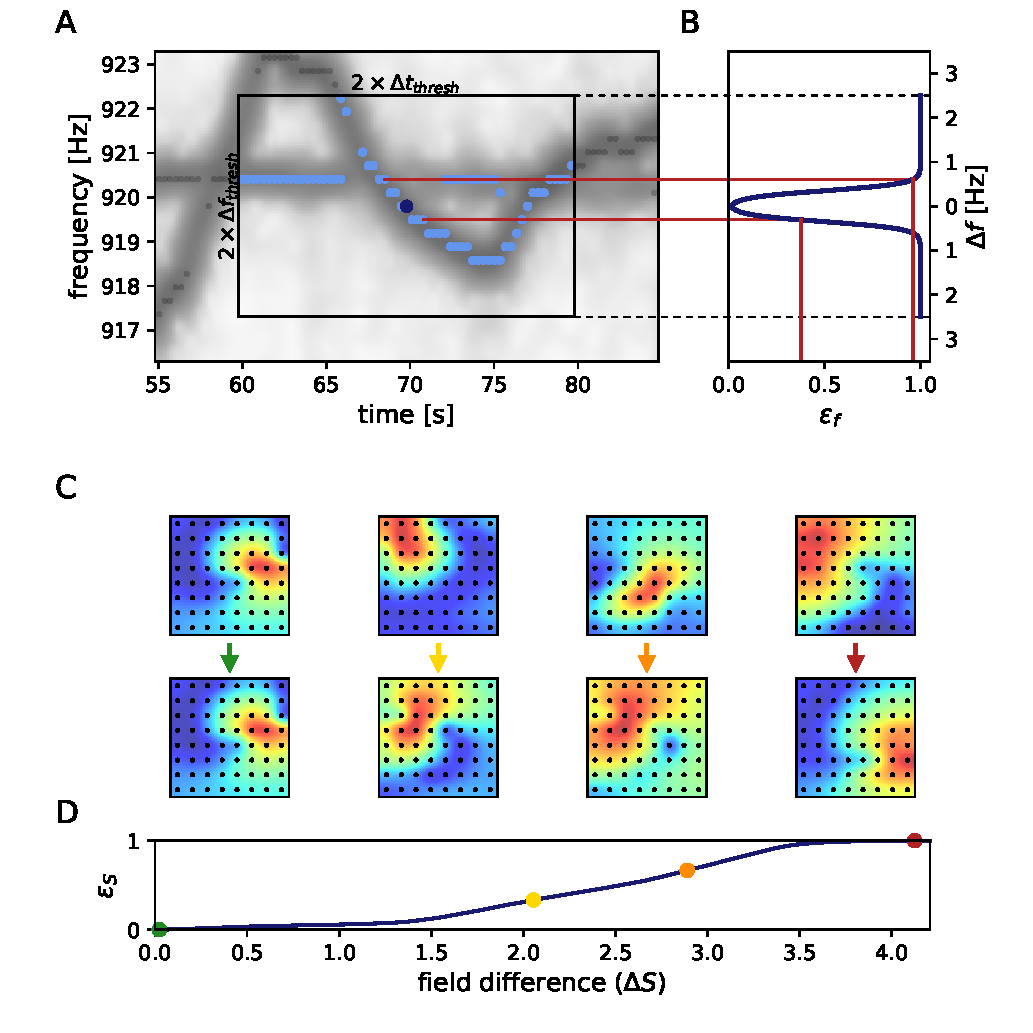
\includegraphics[width=.9\linewidth]{tracking_features_new}}
  \caption{\label{features} Signal errors are estimated to determine tracking order. \figitem{A} For each valid electric fish signal (see \figref{signal_extraction}), potential connection partners are limited by a time difference threshold ($\Delta t_{thresh}$) of $\pm$\,10\,s and a frequency difference threshold ($\Delta f_{thresh}$) of $\pm$\,2.5\,Hz. For a given signal (dark blue), potential connection candidates (light blue) need to be within these thresholds (box), whereas signals beyond these thresholds (grey dots) are rejected as potential connections. \figitem{B} Frequency differences are translated into frequency errors ($\varepsilon_{f}$) using a sigmoid function (\eqnrefb{errpr_eodf_eq}) favoring smaller frequency divergences. \figitem{C} The power distribution of a detected signal across all electrodes represents the basis for the second tracking parameter. The Euclidean distance of powers across electrodes between potential signal pairs (columns) represents the field difference ($\Delta S$, \eqnrefb{field_diff_eq}). With decreasing similarity (columns left to right) the field difference increases. \figitem{D} To obtain normalized field errors ($\varepsilon_{S}$) in the range of the frequency errors ($\varepsilon_{f}$), a given field difference is set into perspective to a representative distribution of field differences obtained by collecting all potential field differences of a manually selected 30\,s window in the recording.}
\end{figure}

\subsection{Identification of potential signal pairs}

The first fundamental assumption of the algorithm described below limits potential signal partners $\beta$ to a signal $\alpha$ by a maximal detection time difference of $\pm$10\,s and maximal EODf difference of $\pm$2.5\,Hz (\subfigref{features}{A}). To assess the similarity between each potential signal pair, we compare signal features ($\vec{X_{k, i}}$, \eqnrefb{signal_features}) by computing a signal error ($\varepsilon_{signal}$) as described below.

\subsubsection{Signal feature - EOD frequency}
As a first tracking feature we utilize the EODf difference 
\begin{equation}\label{f_difference}
\Delta f_{\alpha_i, \beta_j} = | f_{\alpha_i} - f_{\beta_j} |
\end{equation}
between signals with $f_{\alpha_i}$ as the EODf of signal $\alpha$ detected at time $i$ and $f_{\beta_j}$ of signal $\beta$ detected at time $j$ respectively. The EODf of electric fish represents one of the most stable natural oscillator known \citep{Moortgat1998} and has therefore already previously been used to track signals of electric fish \citep{Henninger2020}. Individual EODfs stay remarkably stable over a magnitude of minutes to hours. However, small fluctuations ($\leq$\,200\,mHz) can, first, occur naturally and, second, be an artifact of EODf detection in PSDs. Larger EODf differences, however, indicate either the occurrence of a (comparatively uncommon) communication signal (e.g. \citealp{Zupanc2002, Triefenbach2008, Raab2021}) or signals originating from different individuals. In order to adequately evaluate whether the EODf difference between a signal $\alpha$ and $\beta$ indicates them to originate from the same or different individuals, we compute a frequency error using a logistic function 
\begin{equation}\label{errpr_eodf_eq}   
  \varepsilon_{f}(\Delta f) = \frac{1}{1 + e^{-\frac{\Delta f - f_0}{df}}}
\end{equation}
with $\Delta f$ representing the EODf difference between the corresponding signals (\eqnrefb{f_difference}), $f_0 = 0.35$\,Hz being the frequency-offset and turning point of the logistic function, and $df = 0.08$\,Hz its corresponding slope (\subfigref{features}{B}). Applying this transformation, we mitigate the effect of small frequency differences ($\Delta f$) and equalize larger frequency differences in the assessment of whether two signals $\alpha$ and $\beta$ originate from the same or different individuals. 

\subsubsection{Signal feature - Electric field properties}

EODf traces of electric fish occasionally cross each other, e.g. when individuals actively alter their EODf in the context of communication (e.g. \citealp{Zupanc2002, Triefenbach2008, Raab2021}, \subfigrefb{features}{A}). Here, frequency as a tracking feature potentially results in flawed connections. Therefore, we utilize the spatial properties of a signal, i.e. signal powers across recording electrodes, as a complementary second tracking parameter reflecting the position and orientation of a fish (\citealp{Madhav2018}, \subfigrefb{features}{C}). The spatial properties 
\begin{equation}\label{field_properties}
S_{k, i}(x) = \frac{L_{k, i}(x) - L_{k, i_{min}}}{L_{k, i_{max}} - L_{k, i_{min}}}
\end{equation}
of a signal $k$ detected at time $i$ are the logarithmic signal powers ($L_{k, i}(x)$) extracted from the power spectrum of the respective electrode $x$ at the signal's frequency ($f_{k, i}$) normalized across recording electrodes by their smallest value 
\begin{equation}
L_{k, i_{min}} = \min_x L_{k, i}(x)
\end{equation}
and largest value ($L_{k, i_{max}}$) respectively. 

We compare the spatial properties of signals by computing their Euclidean distance 
\begin{equation}\label{field_diff_eq}
  \Delta S_{\alpha_i, \beta_j} = \sqrt{\sum_{x=1}^{n} (S_{\alpha_i}(x) - S_{\beta_j}(x))^2}
\end{equation} 
with $S_{\alpha_i}(x)$ and $S_{\beta_j}(x)$ being the normalized logarithmic powers extracted from the respective PSDs of electrodes $x$ at the frequencies $f_{\alpha_i}$ and $f_{\beta_j}$ of the respective signals  $\alpha_i$ and $\beta_j$. However, this arbitrary field difference ($\Delta S$) is heavily dependent on the configuration of the recording setup, especially on the number of recording electrodes used. To circumvent this issue and obtain field errors independent from the number of electrodes used in different recording setups, we define the field error 
\begin{equation}
\varepsilon_S(\Delta S_{\alpha_i, \beta_j}) = \int_0^{\Delta S_{\alpha_i, \beta_j}} p(\Delta S)\,d\Delta S
\end{equation}
 between the field properties $S_{\alpha_i}$ of signal $\alpha_i$ and $S_{\beta_j}$ of signal $\beta_j$ as the ratio of field differences in a representative field difference distribution ($p(\Delta S)$) smaller than the respective field difference to assess (\subfigref{features}{D}). To obtain this representative distribution of field differences ($p(\Delta S)$), we select a 30\,second data snippet within the respective data-set where fish can be assumed to be active (i.e. during night time) and compute the field differences for each potential signal pair ($\Delta t_{\alpha, \beta} \leq\pm$\,10\,s). 


\subsubsection{The compound signal error}

With the approach described above, we obtain for each signal pair a frequency error ($\varepsilon_{f}$) and field error ($\varepsilon_{S}$) ranging from 0 to 1. Finally, we compute the compound signal error ($\varepsilon_{signal}$) to quantify the overall disparity of signals using the formula
\begin{equation}\label{sig.error} 
  \varepsilon = \frac{2}{3} * \varepsilon_{S} + \frac{1}{3} * \varepsilon_{f}
\end{equation}
where we double weight the field error ($\varepsilon_{S}$) and single weight the frequency error ($\varepsilon_{f}$). This is because tracking issues usually arise from low $\varepsilon_{f}$. Nevertheless, $\varepsilon_{f}$ remains to be a relevant tracking feature, especially when fish are in close proximity (low $\varepsilon_{S}$).

\subsection{Snippet tracking}

\begin{figure}[t]
  \centerline{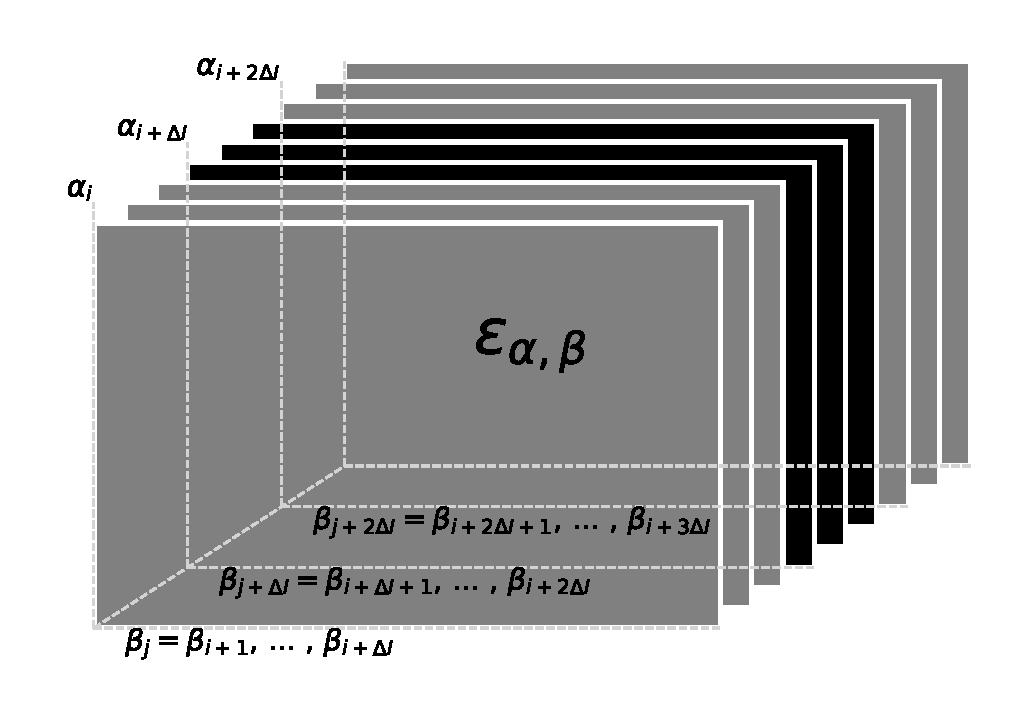
\includegraphics[width=.9\linewidth]{cube_error}}
  \caption{\label{error_cube} Error cube containing all signal errors ($\varepsilon_{\alpha, \beta}$) for possible signal pairs $\alpha$ and $\beta$ within the current tracking window. Each layer, referring to a time step $i$, contains the signal errors between all signals $\alpha_i$ detected at this time-step $i$ and their potential signal partners $\beta_j$ detected maximally 10\,s after signal $\alpha_i$ ($\Delta I$ time-steps after signal $\alpha_i$). Signal errors in grey layers correspond to signal pairs where one signal partner could potentially show a smaller signal error to a signal outside the error cube. Only connections based on the signal errors in the black layers can be assumed to be valid since all potential connections of both signal partners are within the error cube. Connections established in the 1$^{st}$ level tracking based on signal errors in black layers are appended to signal traces of previous tracking steps in the 2$^{nd}$ level tracking.}
\end{figure}

In order to reduce computation time and power without impairing tracking accuracy, we initially only track signals in snippets of 30\,seconds at a time (\figref{tmp_tracking}). Within these tracking windows, we first compute signal errors ($\varepsilon$) between each potential signal pair $\alpha$ and $\beta$ and store the corresponding signals errors in a three-dimensional error cube where the first two dimensions refer to signals $\alpha_i$ and $\beta_j$ and the third dimension to the time step $i$ where signals $\alpha_i$ have been detected (\figref{error_cube}). Connections between signal pairs are then established according to the order of signal errors stored in the error cube starting with the smallest 
\begin{equation}\label{min_e_signal_connect}
  \min \; \varepsilon_{\alpha, \beta}, \; \alpha \in \alpha_i,\;\dots,\;\alpha_{i + 2\Delta I}, \; \beta \in \beta_j,\;\dots,\;\beta_{j + 3\Delta I}, \; i \leq j \leq i + \Delta I  
\end{equation}
representing those signals $\alpha_i$ and $\beta_j$ most likely to originate from the same individual (\figref{tmp_tracking}). Depending on the signal pair and previously established connections, signal traces are established, appended, or joined. Connections are only valid and formed in the absence of temporal conflicts, i.e. a signal trace cannot feature two signals at the same time. As a result, we obtain signal traces build upon minimal signal errors within a 30\,seconds tracking window. 

However, since signals within the first and last 10\,seconds of a tracking window can potentially show lower signal errors to disregarded signals outside the current tracking window, these connections are potentially flawed (grey layers in \figref{error_cube}; grey bars in \figref{tmp_tracking}). Only connections established within the central 10\,seconds regard all other potential signal partners and can therefore be assumed to be valid. Accordingly, only the section of assembled signal traces corresponding to these central 10\,seconds of the current tracking window are further processed in the 2$^{nd}$ order tracking, where they are appended to already validated, previously detected signal traces (\figref{running_connection}). 

\begin{figure}[t]
  \begin{minipage}[t]{0.4\textwidth}\mbox{}\\[-2ex]
    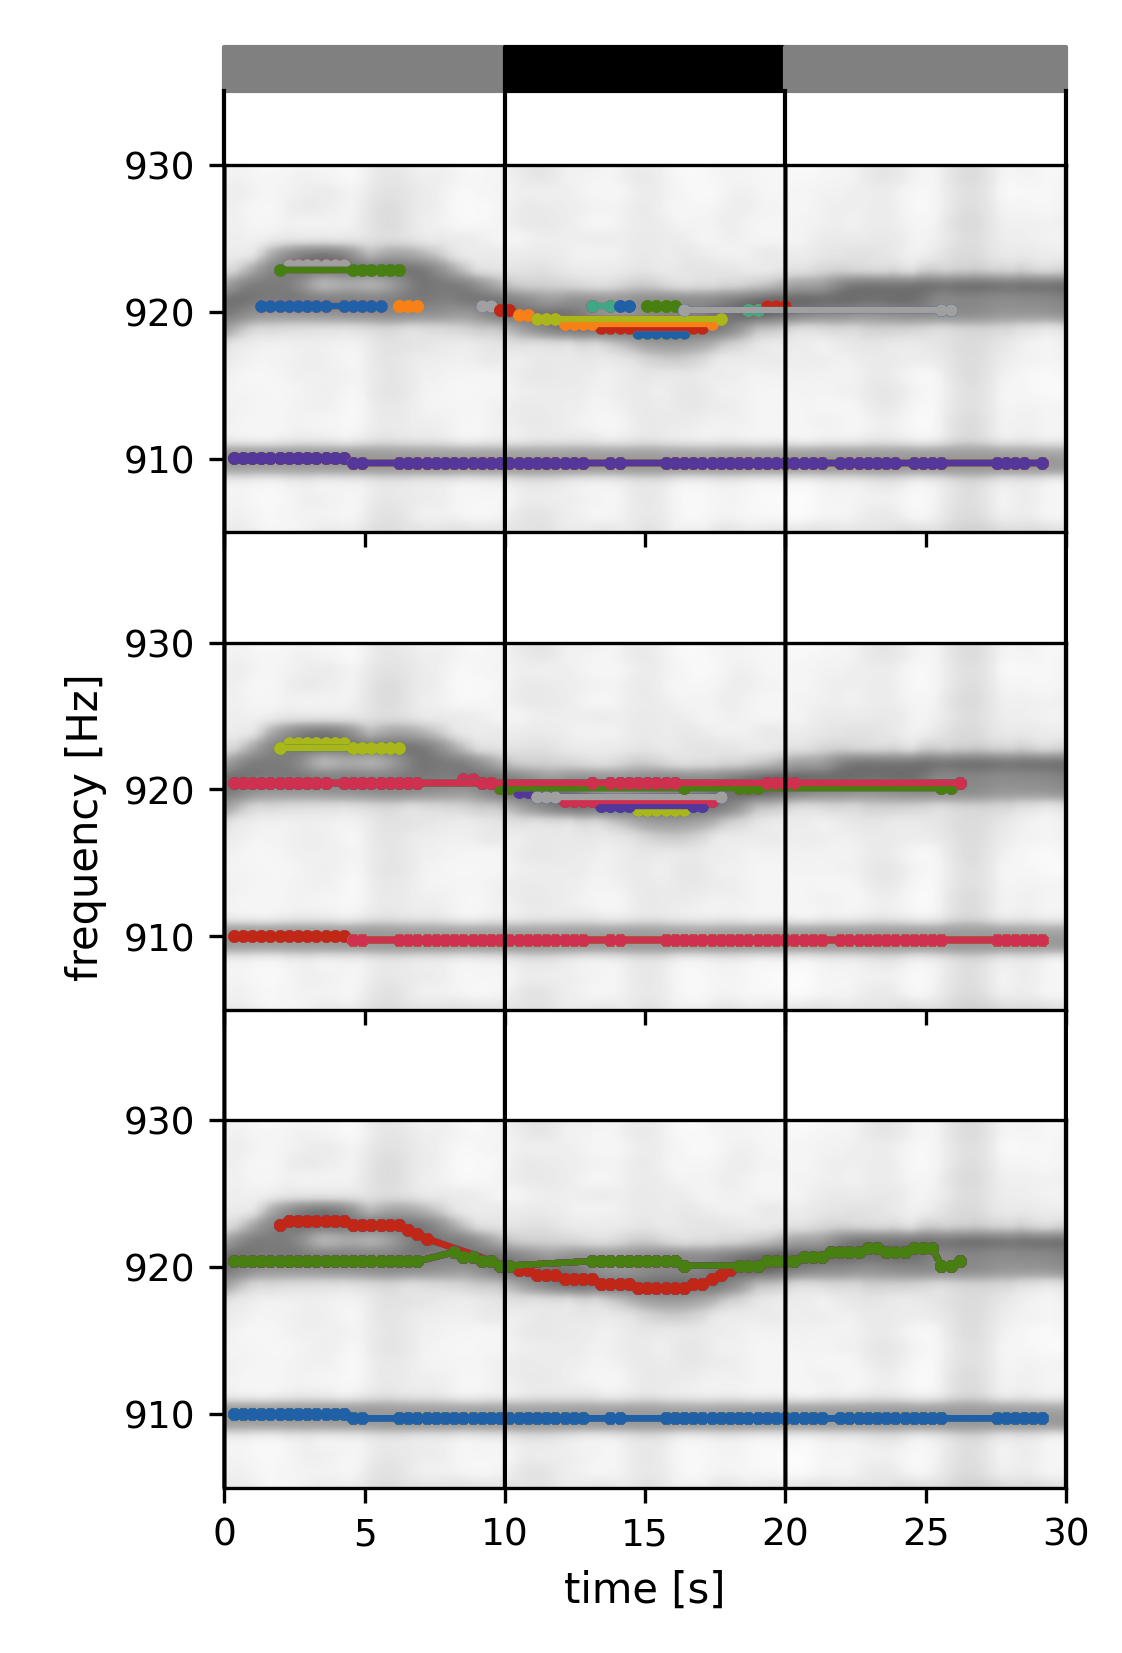
\includegraphics{tmp_ident_tracking}
  \end{minipage}
  \hfill
  \begin{minipage}[t]{0.38\textwidth}
  \caption{\label{tmp_tracking} 1$^{st}$ level signal tracking. Signals detected in  30\,s data snippets are connected to each other and assigned to fish identities according to their signal error. Signal pairs with smaller signal errors are connected first. With increasing signal error, more connections and identities are formed, complemented, or merged when no interference with already established connections emerge (no temporal overlap). Different stages of the 1$^{st}$ level tracking are shown in the three panels. While multiple separate signal traces are still present in the upper panels (different colors), only three EODf traces corresponding to three individual fish are left with the completion of the 1$^{st}$ level snippet tracking (bottom panel). Since each signal can potentially establish a best connection to a target signal in a range of $\pm$10\,s, only signal pairs within the central 10\,s of each 30\,s data snippet regarded all potential signal partners and are assumed to be valid. EODf traces in these central 10\,s are assigned to other EODf of previous tracking iterations.}
  \end{minipage}
\end{figure}

\subsection{Snippet assembly}
The assembly of the 10\,seconds signal traces obtained in the 1$^{st}$ level tracking (\subfigref{running_connection}{A}) and validated signal traces from preceding tracking steps (\subfigref{running_connection}{B}) proceeds, similar to the 1$^{st}$ order tracking, based on the smallest signal errors between them. 

To determine the connection order the smallest signal error 
\begin{equation}\label{min_e_snippet_connect}
  \min \; \varepsilon_{\alpha, \beta}, \; \alpha \in \alpha_i,\;\dots,\;\alpha_{i + \Delta I}, \; \beta \in \beta_{j + \Delta I},\;\dots,\;\beta_{j + 2\Delta I}, \; i \leq j \leq i + \Delta I 
\end{equation}
in the error cube between those signals $\alpha$ corresponding to the first 10\,seconds of the current tracking window ($\alpha \in \alpha_i \dots \alpha_{i + \Delta I}$) and signals $\beta$ referring to the central 10\,seconds of the current tracking window ($\beta \in \beta_{i + \Delta I} \dots \beta_{i + 2\Delta I}$) is determined. The 10\,second signal trace extracted in the 1$^{st}$ level tracking containing signal $\beta$ (green dot in \subfigref{running_connection}{C}), is then connected to the final  signal trace (from previous tracking steps) containing signal $\alpha$ (black dot in \subfigref{running_connection}{C}). This step is repeated with signal pairs of increasing signal errors until all possible connections are established (\subfigref{running_connection}{D}). 

The described 1$^{st}$ and 2$^{nd}$ order tracking steps are repeated alternately with data snippets shifted by 10\,seconds until the end of the recording is reached and tracking is finalized. For each tracking iteration, the error cube needs to be updated. Those layers referring to the time steps $i$ to $i + \Delta I$ of the first 10\,seconds of the previous tracking snippet are removed (frontal grey layers in \figrefb{error_cube}) and new layers referring to the next 10\,seconds beyond the last tracking snippet and their signal pairs $\alpha$ and $\beta$ are extended to the error cube in preparation for the next tracking iteration.


\begin{figure}[h!]
  \centerline{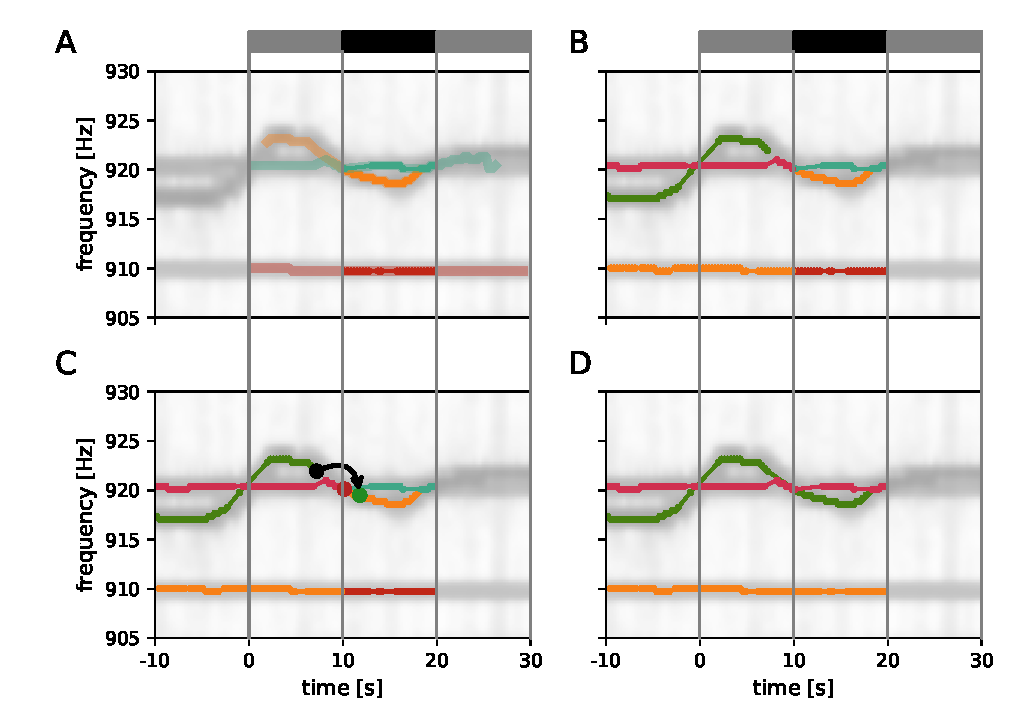
\includegraphics[width=.9\linewidth]{assign_tmp_identities}}
  \caption{\label{running_connection} 2$^{nd}$ level snippet tracking. EODf traces obtained from preceding 1$^{st}$ level tracking are connected to EODf traces of previous tracking steps. \figitem{A} EODf traces obtained from preceding 1$^{st}$ level signal tracking. Only connections within the central 10\,s of these EODf traces (opaque traces; black bar) can be assumed to be valid since signals before and after (faded traces; grey bars) have potential signal partners not accounted for in the 1$^{st}$ level signal tracking of the corresponding tracking window. \figitem{B} Additional display of EODf traces of previous tracking iterations. \figitem{C} EODf traces are connected according to the smallest possible signal error between any signal traces. The signal error between the origin signal (black) and the target signal (green) represents the smallest signal error between signal traces, which leads to the conjunction of the corresponding green and orange EODf traces. An alternative signal (red) has a larger signal error to the origin signal. \figitem{D} Connected EODf traces which will be extended in the next tracking iteration. }
\end{figure}

\subsection{Validation of signal traces}

Even though the developed algorithm is capable of tracking EODs of electric fish with unequalled accuracy (see below), occasional tracking errors still remain. We developed a GUI based software to visually inspect and validate tracked EODf traces and fix flawed connections (\figref{GUI}). Flawed connections can easily be identified by their clear deviation from the spectrogram displayed in the background. Furthermore, signal traces with a detection gap beyond the threshold of the tracking algorithm can be manually connected based on visual cues from the spectrogram. The resulting validated signal traces are then stored and analyzed depending on an experimental hypothesis \citep{Raab2019, Raab2021}.

\begin{figure}[h!]
  \centerline{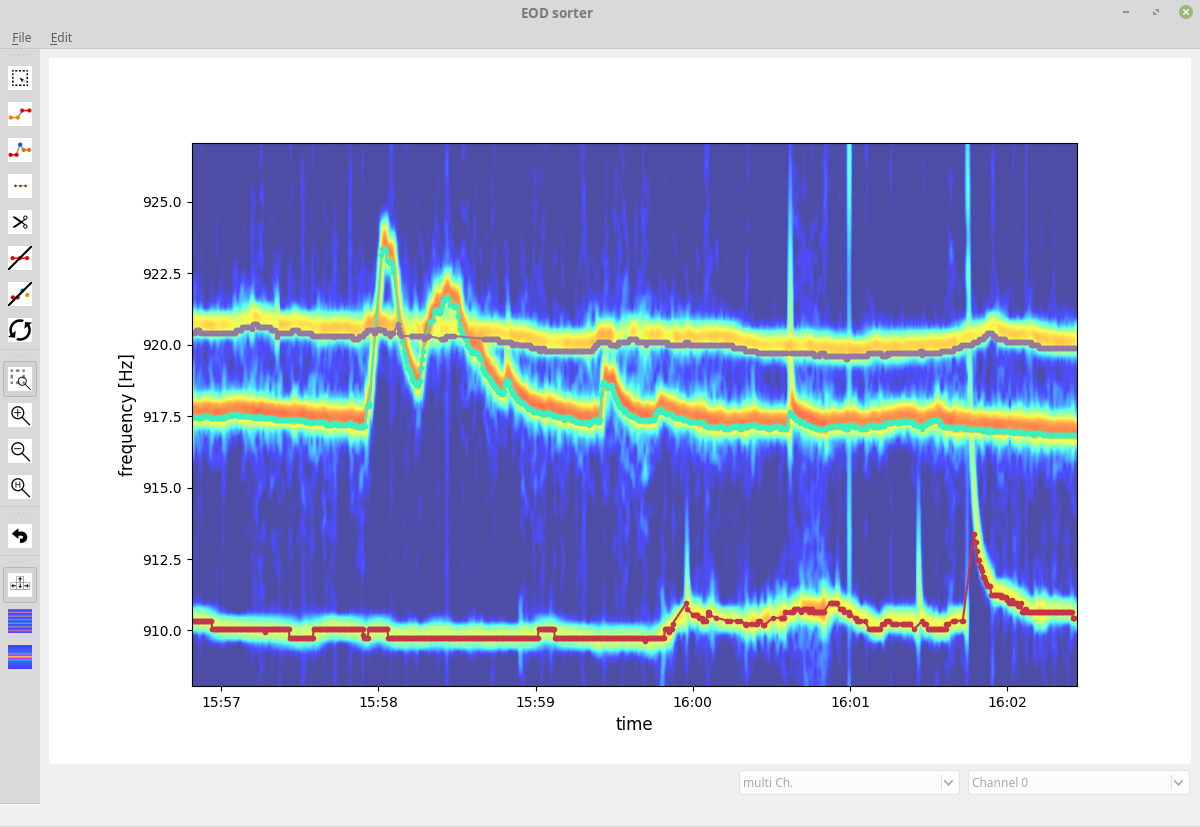
\includegraphics[width=.9\linewidth]{signal_tracker_GUI}}
  \caption{\label{GUI} Graphical user interface of the custom software developed to visually validate tracked signal traces and fix occasionally occurring flawed connections. The user is presented with the tracked signal traces (EODf traces) displayed on top of a summed up spectrogram, e.g. spectrograms added up across recording electrodes. The user can delete, cut, and connect signal traces or delete signals corresponding to electric noise.}
\end{figure}

\section{Detection and evaluation of tracking conflicts}

In order to quantify the accuracy of the presented tracking algorithm, we re-tracked signals of a whole population of \lepto{} recorded with an 8$\times$8 recording electrode grid in a small stream in the Llanos of Colombia during the day of 10$^{th}$ of April, 2016. During the tracking progress, connections established by the 1$^{st}$ level snippet tracking (\figref{tmp_tracking}) are compared to signal traces of the same recording after being visually inspected, corrected, and validated in post-processing using the GUI based Software (checked signal traces, \figref{GUI}). For each valid connection formed during the 1$^{st}$ level snippet tracking, i.e. when both signals $\alpha$ and $\beta$ are within the central 10\,seconds of the current tracking window, we determine whether a potential tracking conflict exists, e.g. if potential signal partners $\beta$ are associated with different checked signal traces. For each potential tracking conflict, we extract the EODf difference ($\Delta f$), field property difference ($\Delta S$), frequency error ($\varepsilon_f$), field error, ($\varepsilon_S$), and compound signal error ($\varepsilon$) between signal $\alpha$ and the best signal partner $\beta$ (smallest signal error $\varepsilon$) associated with the same checked signal traces (true connection), as well as between signal $\alpha$ and the best signal partner $\beta$ belonging to an alternative checked signal trace (false connection). 
%By comparing signal differences and error between true and false connections we are able to determine their suitability as tracking features (\figsref{signal_diff}, \fref{signal_error}).  

\section{Tracking feature quality assessment}

\begin{figure}[t]
  \begin{minipage}[t]{0.4\textwidth}\mbox{}\\[-2ex]
    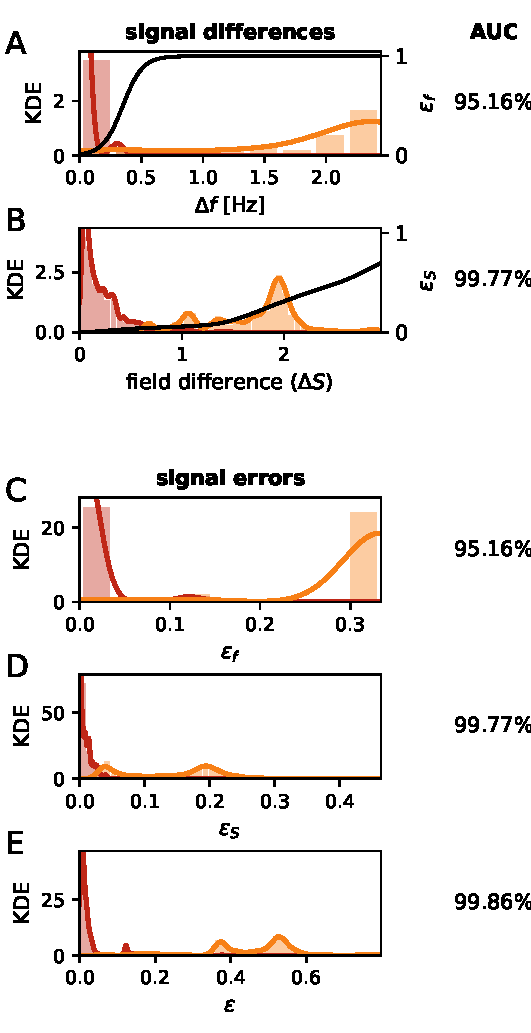
\includegraphics{signal_diff_error}
  \end{minipage}
  \hfill
  \begin{minipage}[t]{0.35\textwidth}
  \caption{\label{signal_diff_error} Often signals can potentially be assigned to multiple different signal traces of different fish (identified \textit{post hoc}). Smaller signal feature differences and errors to the origin signal indicate correct target signals (red). Signal differences and errors are larger for the alternative target signals (orange). \figitem{A} EODf differences are smaller to target signals than alternative signals. However, distributions overlap as quantified by a ROC-analysis (AUC$=$95.16\,\%). A sigmoid function (black) is used to translate EODf difference to frequency errors ($\varepsilon_{f}$). \figitem{B} Also field differences to target signals are smaller than to alternative signals. However, the overlap of corresponding distributions is smaller (AUC$=$99.77\,\%). The function translating field differences to field errors ($\varepsilon_{S}$) as described in \subfigref{features}{D} is shown in black. \figitem{C, D, E} Frequency error ($\varepsilon_{f}$, \panel~C), field error ($\varepsilon_{S}$, \panel~D), and compound signal error ($\varepsilon$, \panel~E) of origin signals to correct target signals (red) and alternative signals (orange). Frequency and field errors (C, D) resemble scaled signal differences (A, B) and are therefore equally suitable as tracking features (equal AUC). However, the compound signal error incorporating both field and frequency error is the most suitable for tracking electric fish signals and is therefore utilized in the presented algorithm (AUC$=$99.86\,\%).
  }
  \end{minipage}
\end{figure}

%\begin{figure}[h!]
%  \centerline{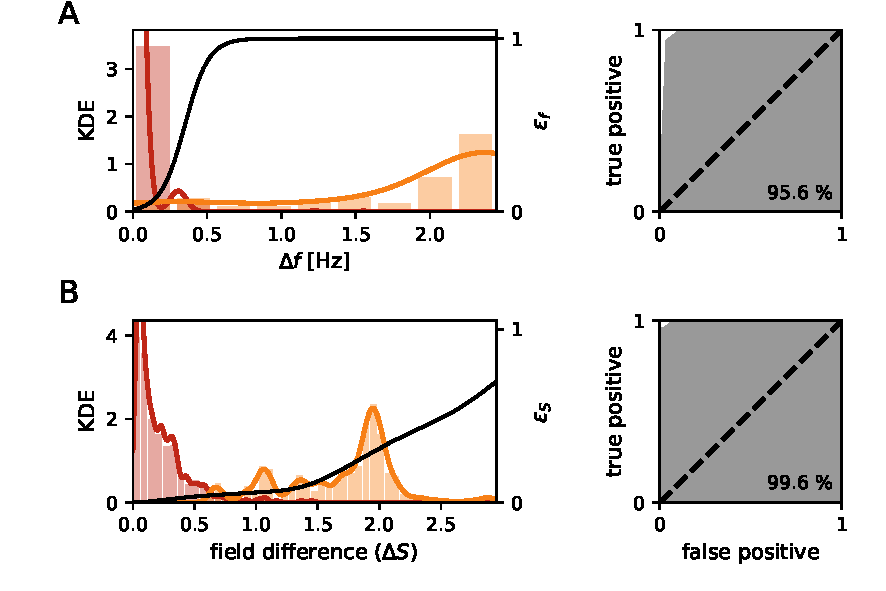
\includegraphics[width=.9\linewidth]{freq_field_difference}}
%  \caption{\label{signal_diff} Often a origin signal could potentially be assigned to signal traces originating from different fish (identified \textit{post hoc}). Different signal attribute differences vary depending on whether the origin signal is compared to the real, correct target signal (red) or the alternative potential signal partner (orange). \figitem{A} EODf difference are smaller to target signals before alternative signals. However, distributions overlap as quantified by a ROC-analysis (AUC$=$99.0\,\%, right panel). A sigmoid function (black) is used to translate EODf difference to frequency errors ($\varepsilon_{f}$). \figitem{B} Also field differences are smaller to target signals before alternative signals with a smaller overlap in distributions (AUC$=$99.6\,\%). The function translating field differences to field errors ($\varepsilon_{S}$) as described in \subfigref{features}{D} is shown in black.}
%\end{figure}

In order to assess the potential of each signal feature difference ($\Delta f$ \& $\Delta S$) and error ($\varepsilon_f$, $\varepsilon_S$, $\varepsilon$) to indicate true and false connections, we determine the area under the curve (AUC) of a receiver-operating characteristic between true and false connections as well as the proportion of signal differences/errors of true connections being smaller than those of the corresponding false connections (\figref{signal_diff_error}). While tracking a full data-set recorded during the day of the 10$^{th}$ of April, 2016, $261\,344$ potential tracking conflicts were detected and are evaluated in the following. To highlight the capabilities of the presented tracking algorithm, we first evaluate only those tracking conflicts corresponding to a 5\,minute snippet being especially challenging to track because of several crossing EODf traces. A representative segment of this 5\,minute data snippet is displayed in \figref{GUI} and is the basis for \figsref{signal_extraction}, \fref{features}, \fref{tmp_tracking} and \fref{running_connection}

The least reliable tracking feature appears to be an individual's EODf ($\Delta f$/$\varepsilon_f$). Regarding only tracking conflicts corresponding to the challenging to track 5\,minute data snippet, frequency differences/errors of true connections were smaller in only 94.83\,\% (440/464) of the cases and the comparison of frequency difference/error distributions between true and false connections using a ROC-analysis resulted in an AUC of 95.16\,\% (\subfigref{signal_diff_error}{A, C}). Better results can be achieved utilizing the field property differences ($\Delta S$/$\varepsilon_S$) as tracking feature. For the tracking conflicts corresponding to the challenging to track 5\,minute data snippet, field property differences of true connections were smaller in 99.57\,\% (462/464) of the cases and the AUC from the ROC-analysis describing the difference between the distributions of field differences/errors between true and false connections already reached 99.77\,\% (\subfigref{signal_diff_error}{B, D}). However, these results can even be surpassed when utilizing a compound signal error ($\varepsilon$) combing both frequency error ($\varepsilon_f$) and field error ($\varepsilon_S$). In 99.87\,\% (462/464) of the tracking conflict corresponding to the 5\,minute data snippet, true connections had smaller compound signal error ($\varepsilon$) than false connections. The associated ROC-analysis evaluating the difference between signals errors of true and false connections resulted in an AUC of 99.86\,\% (\subfigref{signal_diff_error}{E}). 

Regarding all tracking conflicts of the whole recording, similar observations could be made. However, the higher proportion of ``easy'' tracking conflicts led to a shift of tracking feature accuracy to higher values and differences between them were less pronounced. Nevertheless, EODf still remained to be the least favorable tracking parameter (99.73\,\% smaller frequency errors in true connections than in false connections; AUC = 99.79\,\%) followed by the field difference (99.81\,\% smaller frequency errors in true connections than in false connections; AUC = 99.85\,\%). The best results could be achieved when utilizing the compound signal error for tracking (99.95\,\% smaller frequency errors in true connections than in false connections; AUC = 99.98\,\%).


\section{The advantages of the presented algorithm}

Previous approaches on tracking EODs of individual wave-type electric fish either utilized their EODf \citep{Henninger2020} or the spatial properties of their electric fields \citep{Madhav2018} as tracking features. We assessed how suitable both signal features alone  as well as a combination of both (compound signal error: $\varepsilon$, \eqnrefb{sig.error}) are for tracking by evaluating tracking conflicts occurring while processing a recording of a natural, high density population of \lepto{} in a stream in Colombia. 

According to this evaluation, the comparison of spatial field properties ($\Delta S$) achieves a higher tracking accuracy than EODf comparison ($\Delta f$). Certainly, the EODf of \lepto{} can be remarkably stable over minutes to hours \citep{Moortgat1998}. However, \lepto{} frequently alters its EODf actively in the context of electrocommunication \citep{Smith2013}. Accordingly, the suitability of EODf as tracking feature decreases the more fish are recorded and analyzed simultaneously since EODf differences between fish are potentially smaller and interactions between fish involving active EODf alterations can be assumed to be more frequent. Therefore, spatial field properties resembling a fish's spatial position and orientation represent a more honest and suitable tracking feature, especially when only those signal pairs with small EODf differences ($\Delta f$) are regarded for comparison and tracking.

Nevertheless, the highest tracking accuracy can be achieved by utilizing a compound signal error ($\varepsilon$) comprising both EODf difference ($\Delta f$) and spatial field property difference ($\Delta S$) as tracking feature. This is because the compound signal error ($\varepsilon$) implements a tracking bias that helps to resolve tracking conflicts in the event of crossing EODf traces. In such intersections, temporarily only one signal can be extracted by detecting peaks in the compound PSD (e.g. \subfigref{features}{A}). Since the spatial properties ($S$) of these overlaid signals comprise the electric field properties of both individual signals, their assignments are only correct at chance level when solely the signals' spatial field properties are utilized for tracking. The compound signal error ($\varepsilon$), on the other hand, slightly favors connections of signal pairs with more similar EODfs resulting in a bias for overlaid signals detected in EODf trace interactions to be connected to the EODf traces of those fish not altering their EODf (\figref{tmp_tracking}, green trace in bottom panel). The other signal traces, accordingly, remain to be connected across the intersection afterwards. 

The advantage of the presented tracking algorithm not only rests upon the utilization of a compound signal error as tracking feature, but also on the tracking method itself. When studying animals and their behaviors by means of evaluating external recordings, we rely on the detection of sensory cues emitted actively or passively by the animals themselves \citep{Dell2014, Hughey2018}. In cluttered environments or when signals are weak (low signal-to-noise-ratio), reliable signal detection is often impaired and detection losses frequently occur. These detection gaps complicate reliable tracking, especially when signals are tracked according to their temporal occurrence. In recordings of electric fish, detection losses frequently result from fish being too far away from recording electrodes or electric field being blocked by any objects between fish and recording electrode. However, associated tracking issues can be avoided with the presented algorithm since it is less reliant on the temporal detection of signals, but connections are rather established according to the smallest signal errors in discrete tracking windows.

\section{Conclusion}

The electric field of \lepto{} poses a great opportunity for studying natural behaviors of electric fish in freely moving and interacting populations. The EODs of whole groups can be recorded simultaneously by means of recording electrode arrays submerged in the water and tracked for individual fish using different EOD characteristics. With the presented algorithm, we combine previous approaches of tracking either the individual specific EODf \citep{Henninger2020} or the spatial properties of electric fields resembling a fish's spatial location and orientation \citep{Madhav2018}. We use a compound signal error incorporating both EODf and spatial field property difference and obtain EOD traces of individual fish by assembling signals in discrete tracking windows according to the order of increasing signal errors. With this approach, our algorithm improves in resolving various tracking issues, e.g. resulting from crossing EODf traces or detection losses, and enables EOD tracking with unprecedented accuracy. Since tracked EOD traces allow insights into various behavioral aspects of electric fish, including communication and movement, our algorithm is applicable in a broad range of behavioral studies. It also facilitates high throughput studies including long term behavioral observation since the increased tracking accuracy decreases the expense of extensive EOD trace post-processing. This has already been demonstrated in an experiment evaluating the spatio-temporal movements of a group of 14 \lepto{} in the context of an individual's social status \citep{Raab2019} as well as in an experiment investigating the communication behavior of pairs of \lepto{} competing over a shelter during staged competition \citep{Raab2021}.
%\bibliography{journalsabbrv,references}
%\figurecaptions

%\bibliographystyle{jneurosci}
%\bibliography{../journalsabbrv,../references}

